%!TEX root = ../template.tex
%%%%%%%%%%%%%%%%%%%%%%%%%%%%%%%%%%%%%%%%%%%%%%%%%%%%%%%%%%%%%%%%%%%
%% chapter1.tex
%% NOVA thesis document file
%%
%% Chapter with introduction
%%%%%%%%%%%%%%%%%%%%%%%%%%%%%%%%%%%%%%%%%%%%%%%%%%%%%%%%%%%%%%%%%%%

\typeout{NT FILE background.tex}%

\makeatletter
\newcommand{\ntifpkgloaded}{%
  \@ifpackageloaded%
}
\makeatother

\chapter{Background}
\label{cha:Background}

This section aims to provide information and context on the current state of topics related to the research, including Requirements Engineering, Ethics, 
Large Language Models, and Systematic Mapping Studies. Which serve as the basis for understanding the scope of this research.

\section{Ethics and Ethical Requirements}
The term "ethics" often refers to the investigation and analysis of moral principles and dilemmas. It can be considered as values that encompass the guidelines and standards that govern our decisions in our daily lives,
as well as our emotinoal and conscientious actions.

In the context of ethical software engineering, these values can become actianable through strucutured frameworks that translate the abstract ethical principles into concrete requirements. \cite{spiekermann2022values}

Using the example of a driverless car \cite{guizzardi2023ontology}, several ethical considerations must be taken into account. Beneficence entails ensuring that the car actively creates value 
for its users; for instance, it should select the quickest and safest route to the destination. Non-maleficence requires that the car does not cause harm to its users or others; therefore, 
it must stop whenever an object is in its path to prevent accidents and should exhibit a defensive driving style to enhance passenger safety. Autonomy requirements ensure that the car adheres 
to traffic laws, calculates the best route without human intervention (unless requested by the user), and cannot change the destination without the user’s approval. Explicability, meaning that 
the car should be able to provide explanations for its actions. It needs to clarify why it chose a particular route or decided to overtake another vehicle. In summary, it should be transparent 
in its decision-making, especially in situations where it could put someone at risk.

\subsection{Ethical Principles}
There are several ethical guidelines published by different organizations, institutions and researchers. ECCOLA, a card-based tool to help stakeholders identify and discuss ethical requirements in software 
development \cite{VAKKURI2021111067}, is based on the IEEE Ethically Aligned Design guidelines\footnote{IEEE Ethical Guidelines: \url{https://standards.ieee.org/industry-connections/activities/ieee-global-initiative/}} and 
the EU Trustworthy AI guidelines\footnote{EU AI Guidelines: \url{https://digital-strategy.ec.europa.eu/en/library/ethics-guidelines-trustworthy-ai}}.

\paragraph{IEEE Ethical Guidelines for Intelligent Systems\\}
The ethical and values-based design, development, and deployment of autonomous and intelligent systems (A/IS), acccording to the IEEE Ethical Guidelines for IS, should adhere to the following general principles:

\begin{enumerate}
    \item \textbf{Human Rights}\\
    Autonomous and intelligent systems shall be designed, developed, and operated in a manner that respects, promotes, and safeguards internationally recognized human rights.
    
    \item \textbf{Well-being}\\
    The enhancement of human well-being shall serve as a fundamental criterion for the development of autonomous and intelligent systems.
    
    \item \textbf{Data Agency}\\
    Developers of autonomous and intelligent systems shall empower individuals by ensuring their ability to access and securely share their personal data, thereby preserving their control over their identity.
    
    \item \textbf{Effectiveness}\\
    The creators and operators of autonomous and intelligent systems shall provide demonstrable evidence of their effectiveness and suitability for their intended purpose.
    
    \item \textbf{Transparency}\\
    The rationale underlying any decision made by an autonomous and intelligent system should always be discoverable and comprehensible.
    
    \item \textbf{Accountability}\\
    Autonomous and intelligent systems shall be designed and operated in a manner that ensures clear and unambiguous justification for all decisions made.
    
    \item \textbf{Awareness of Misuse}\\
    Developers of autonomous and intelligent systems shall take proactive measures to mitigate potential misuse and operational risks.
    
    \item \textbf{Competence}\\
    Developers shall define, and operators shall adhere to, the requisite knowledge and skill levels necessary for the safe and effective operation of autonomous and intelligent systems.
\end{enumerate}

\paragraph{EU Trustworthy AI guidelines\\}
Based on the EU trustworthy AI guidelines, AI systems must adhere to the following key requirements:

\begin{enumerate}
  \item \textbf{Human Agency and Oversight}\\
  AI systems should empower human beings, allowing them to make informed decisions while fostering their fundamental rights. Proper oversight mechanisms must be in place, which can be achieved through human-in-the-loop, human-on-the-loop, and human-in-command approaches.
  
  \item \textbf{Technical Robustness and Safety}\\
  AI systems must be resilient and secure, ensuring fallback plans in case of failures. They should be accurate, reliable, and reproducible to minimize and prevent unintended harm.
  
  \item \textbf{Privacy and Data Governance}\\
  AI systems must fully respect privacy and data protection while implementing robust data governance mechanisms. This includes ensuring data quality, integrity, and legitimized access to data.
  
  \item \textbf{Transparency}\\
  AI systems should maintain transparency in data usage, system operations, and business models. Traceability mechanisms should be implemented to achieve this. Additionally, AI decisions should be explained in a stakeholder-adapted manner, and humans must be made aware of AI interactions and system capabilities.
  
  \item \textbf{Diversity, Non-Discrimination, and Fairness}\\
  AI systems must prevent unfair biases that could marginalize vulnerable groups or exacerbate discrimination. They should be accessible to all individuals, regardless of disability, and involve relevant stakeholders throughout their lifecycle.
  
  \item \textbf{Societal and Environmental Well-being}\\
  AI systems should benefit humanity, including future generations, by ensuring sustainability and environmental friendliness. Their social and societal impacts should also be carefully considered.
  
  \item \textbf{Accountability}\\
  Mechanisms must be established to ensure responsibility and accountability for AI systems and their outcomes. Auditability, which assesses algorithms, data, and design processes, is crucial, particularly in critical applications. Moreover, accessible redress mechanisms should be in place.
\end{enumerate}

On the other hand the authors Mark Ryan and Bernd Stahl, published an impressive list of guidelines for developers and users\cite{ryan2020artificial} to provide guidence  when developing ethically aligned AI systems.
The following are the Key Ethical Principles from Mark Ryan and Bernd Stahl's guidelines:

\paragraph{Transparency}
\begin{itemize}
    \item AI should be transparent in its operation and decision-making process.
    \item Key aspects: explainability, interpretability, communication, disclosure.
    \item AI decisions should be reproducible and subject to external auditing.
\end{itemize}

\paragraph{Justice and Fairness}
\begin{itemize}
    \item AI should promote justice and fairness, avoiding biases and discrimination.
    \item Key aspects: inclusion, equality, non-bias, non-discrimination, accessibility.
    \item AI organizations should implement fairness-aware data processing methods.
\end{itemize}

\paragraph{Non-Maleficence}
\begin{itemize}
    \item AI should be designed to prevent harm to individuals and society.
    \item Key aspects: security, safety, prevention, integrity, protection.
    \item AI should not compromise human well-being or cause social dislocation.
\end{itemize}

\paragraph{Responsibility}
\begin{itemize}
    \item Developers and organizations must take responsibility for AI’s impact.
    \item Key aspects: accountability, liability, integrity, redress mechanisms.
    \item Ethical training and internal auditing should be implemented.
\end{itemize}

\paragraph{Privacy}
\begin{itemize}
    \item AI should uphold privacy and data protection standards.
    \item Key aspects: personal data security, informed consent, data minimization.
    \item Compliance with legal frameworks such as GDPR is essential.
\end{itemize}

\paragraph{Beneficence}
\begin{itemize}
    \item AI should promote social good and well-being.
    \item Key aspects: public benefit, peace, common good, sustainability.
    \item AI should be used to address global challenges such as healthcare and environmental issues.
\end{itemize}

\paragraph{Freedom and Autonomy}
\begin{itemize}
    \item AI should respect human autonomy and decision-making.
    \item Key aspects: consent, liberty, empowerment, choice.
    \item AI should not manipulate individuals or limit personal freedoms.
\end{itemize}

\paragraph{Trust}
\begin{itemize}
    \item AI systems should be trustworthy and reliable.
    \item Key aspects: transparency, safety, accountability.
    \item Organizations should demonstrate security measures to build trust.
\end{itemize}

\paragraph{Sustainability}
\begin{itemize}
    \item AI should be developed with environmental sustainability in mind.
    \item Key aspects: energy efficiency, resource management, ecological impact.
    \item Organizations should prioritize minimizing AI’s environmental footprint.
\end{itemize}

\paragraph{Dignity and Solidarity}
\begin{itemize}
    \item AI should uphold human dignity and social cohesion.
    \item Key aspects: societal bonds, fairness, non-discrimination.
    \item AI should not undermine social structures or democratic values.
\end{itemize}

These ethical principles collectively provide a foundation for the responsible development and deployment of AI systems. While these principles emphasize different aspects - such as human rights, 
transparency, accountability, and fairness - they converge on the common goal of ensuring that AI systems are aligned with societal values and human well-being.

By integrating these ethical considerations into AI developmenet, organizations can build trust, mitigate potential harms, and ensure that AI systems serve as beneficial tools rather than sources of risk.

Although this thesis is focused on a broader scope of software development, ecompassing not only AI systems. The ethical principles outlined above can be adapted and reused to guide the elicitation
and specification of ethical requirements for software products.


\section{Requirements Engineering}
Requirements engineering can be tought as the systematic process of developing requirements by iteratively and cooperatively analyzing a problem, documenting observations in various representation formats, and checking the accuracy
of the understanding gained. This process, which ultimately populates a requirements document, involves addressing a range of questions about the mehods, iterations, participants, documentation standards, and criteria for 
determining when the process is complete and the requirements are suffienctly accurate \cite{macaulay2012requirements}.


% Requirements Engineering (RE) is a core discipline within software and systems engineering that encompasses the activies of eliciting, analyzing, specifying, validating, and managing the requirements for a system.
% Its aim is to ensure that the final product faithfully reflects the needs and constraints of its stakeholders, thereby reducing risks and improving project success. In their seminal work, Nuseibeh and Easterbrook \cite{nuseibeh2000requirements}
% define RE as a systematic process that is vital for aligning software development with stakeholder goals and for preventing costly rework later in the lifecycle.

\subsection{Requirements}
Requirements are the formal statement of what a system must do or the conditions it must satisfy in order to meet the needs of its stakehodlers. In requirements engineering, a requirement is generally understood as a 
necessary condition or capability that a system must posses in order to solve a particular problem or achieve a specified objective \cite{macaulay2012requirements}. Requirements serve as the 
"real-world goals" that guide the subsequent design, implementation, and validation activities in the system's life cycle \cite{nuseibeh2000requirements}.

\subsubsection{Categories of Requirements}
Requirements are typically divided into two broad categories:
\paragraph{Functional Requirements}
These requirements describe behaviours, functions, or services that a system must provide. They answer the "what" of a system's operation - for example, processing transactions, generation reports, or handling user input.

\paragraph{Non-Functional Requirements (NFRs)}
These requirements are also known as quality attributes, which specify how well the system performs its functions \cite{nuseibeh2000requirements}. They include performance, usability, security, and other constraints that influence
the system's overall quality. This categorization helps in balancing the design choices and ensuring that both the capabilities and the performance characteristics of the system are well understood \cite{nuseibeh2000requirements}.

% \subsection{Ethical Requirements}
% Ethical requirements are a specialized subset of software requirements that explicitly address moral, social, and legal considerations during system design and development. 


% Ethical requirements can be considered NFRs 

\subsection{Requirements Elicitation}
Requirements Elicitation is a fundamental stage of requirements engineering that involves gathering, uncovering, and documenting the needs, expectations, and constraints of stakeholders for a software product and turn them into a 
structured set of requirements. By enganging in thorough preparation, using diverse techniques, and iteratively validating findings, organizations can significantly enhance the chances of project success. When done correctly, this
process not only clarifies what needs to be built but also aligns the entire project team around a shared vision, ultimately leading to software that meets user and business needs. \cite{nuseibeh2000requirements}

There are many techniques to elicit requirements such as interviewing stakeholders on one-on-one or group discussions, workshops and brainstorming in collaborative sessions to generate a wide range of ideas, surveys to capture
feedback from a larger audience, and observing directly how users interact with the system \cite{324822, nuseibeh2000requirements}. The results gathered from these techniques are then gathered and further analyzed and validated 
with stakeholders to ensure they reflect true needs. 


% \subsection{User Stories}
% A User Story is a description of an action that a user could perform in a system, with the objective of guiding the development the development of such system \cite{cohn2004user}. These are usually short sentences expressed via 
% natural language that follow a three part user story template that goes as follows: "As a ..., I want to ..., so that ...".

% According to \cite{cohn2004user} a user story consists of three key elements: A written description that aids in planning and serves as a reference, discussions that elaborate on the details of the story, and 
% tests that document specific requirements and help determine when the story is complete.

% \subsubsection{What is a good story?}
% A good story should be independent, negotiable, valuable to users or customers, estimable, small, and testable \cite{cohn2004user}.

% \paragraph{Independent:} Stories shouldn't have to relie on other stories to be completed. Each story should be it's own case having the ability to be completed at any point without needing another story to be completed first.

% \paragraph{Negotiable:} 



\section{Large Language Models \& Generative AI}
Large Language Models (LLMs) are AI systems designed to comprehend, generate, and manipulate human text. They form the foundation of generative AI, a technology that creates new content—such 
as text, images, or even music—by identifying patterns in extensive datasets.

LLMs are constructed using deep neural network architectures, most notably the transformer model as shown in figure \ref{fig:LLM_transformer_arch}. Transformers 
employ self-attention mechanisms that assess the relationships between words in a sentence, allowing the model to grasp context and long-range dependencies within the text  \cite{NIPS2017_3f5ee243}. 
By training on a vast corpus of text, these models learn the structure of language, gaining knowledge about grammar, facts, reasoning patterns, and even the subtle nuances of human communication.

Generative AI, which encompasses LLMs, utilizes this learned language model to produce new, contextually relevant text. When presented with a prompt, an LLM predicts and samples the next word 
(or sequence of words) from a probability distribution, resulting in coherent and often creative outputs.

The process begins with pre-training, wherein the model is exposed to large volumes of text data. During this phase, the model learns to predict the next word in a sentence, which compels it to 
capture patterns of syntax, semantics, and factual knowledge. After pre-training, the model may undergo fine-tuning on task-specific data to further refine its capabilities.

The core of their operation relies on the transformer architecture, which uses an encoder-decoder framework. Both the encoder and decoder consist of multiple identical layers built around 
self-attention mechanisms and feedforward networks. The encoder processes an input sequence, mapping it to a series of continuous representations. In contrast, the decoder generates an output 
sequence autoregressively, predicting one token at a time based on the encoder's output and the previously decoded tokens.
At the heart of the Transformer is the \textit{multi-head self-attention} mechanism. This allows each token to compute weighted relationships with all other tokens in the sequence through scaled 
dot-product attention. As a result, the model efficiently captures long-range dependencies without the need for sequential computation, unlike recurrent networks.
After the self-attention process, the output passes through a position-wise feedforward network, followed by residual connections and layer normalization. These components enhance stability a
nd improve gradient flow. Because the model does not have built-in recurrence or convolution, positional encodings are added to the input embeddings to preserve the information about word order.
In the decoder, masked self-attention ensures that predictions at each step depend only on previously generated tokens, which maintains autoregressive generation. By utilizing parallel 
computation and attention-based representations, the Transformer achieves state-of-the-art performance in tasks such as machine translation, text generation, and language understanding. 
This capability allows it to interpret complex prompts and generate detailed, human-like responses\cite{NEURIPS2020_1457c0d6}.


In simulating human behavior, large language models (LLMs) generate text that not only follows grammatical rules but also reflects human reasoning and stylistic patterns. They can imitate 
various conversational styles, adjust their tone based on context, and even simulate empathy in their responses. Research into emergent abilities has shown that as these models scale up, 
they start to display sophisticated behaviors that were not explicitly programmed. These behaviors can resemble human intuition and creativity \cite{Lockhart2024}. This aspect can be 
particularly useful for extracting ethical requirements from stakeholder descriptions, as ethical requirements tend to be abstract and often require interpretation and discussion.


\begin{figure}[h]
  \centering
  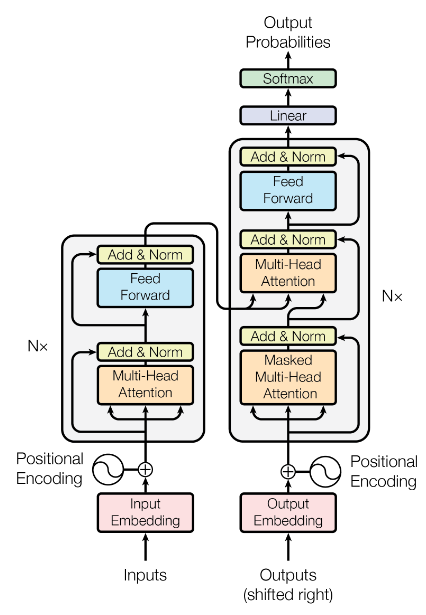
\includegraphics[width=0.5\textwidth]{LLM_transformer_arch}
  \caption{Transformer architecture}
  \label{fig:LLM_transformer_arch}
\end{figure}

\subsection{Generating Personas with LLMs}

The use of LLMs in the generation of personas has gained traction as an effective method for representing diverse user needs and perspectives \cite{10.1145/3643691.3648587}. Personas, as synthetic 
representations of users, are instrumental in requirements engineering, product design, and AI fairness assessments. By leveraging the generative capabilities of LLMs, 
the creation of personas can be automated and diversified, enhancing their applicability in AI systems that require inclusivity and ethical considerations.

\subsubsection{Automating Persona Generation}
Traditional persona creation is a manual process that relies on user research, stakeholder interviews, and demographic analysis. LLMs provide a novel approach by generating detailed, realistic, 
and contextually rich personas based on vast linguistic and social knowledge. Given a set of prompts, an LLM can produce persona profiles that include demographics, behaviors, goals, and potential 
biases. This automation reduces the time and effort required for persona development while increasing the variety and representativeness of personas in AI-driven applications.

\subsubsection{Enhancing Diversity and Inclusion}
A key challenge in AI development is ensuring that systems are designed with inclusivity in mind. LLM-generated personas can be tailored to reflect underrepresented groups, mitigating biases in 
technology development. By conditioning LLM outputs on diverse datasets and ethical guidelines, personas can better represent different socio-economic backgrounds, cultural values, disabilities, 
and intersectional identities.

\subsubsection{Use Cases in AI Requirements Engineering}
The integration of LLM-generated personas into AI development workflows enables a structured method for eliciting diverse requirements. For instance, personas can be used to simulate user interactions, 
assess AI fairness, and guide system testing. In responsible AI engineering, chat-based interactions with virtual personas allow analysts to understand potential ethical concerns before deployment. 
This process contributes to refining AI-driven decision-making and ensuring that user-centric considerations are embedded from the early stages of development.

By harnessing the power of LLMs for persona generation, AI developers can create more representative and ethically responsible AI systems.





\section{Systematic Mapping Study}
An SMS is a type of secondary research method that provides a comprehensive overview by identifying, categorizing, and documenting existing literature \cite{petersen2008systematic}. 
It aids researchers in understanding the scope of a research area, identifying trends, and highlighting gaps in knowledge \cite{almendra2020incremental}. Unlike a Systematic Literature Review (SLR), which seeks to provide a comprehensive and 
detailed synthesis of findings related to a well-defined research question \cite{bombonatti2016usability}, an SMS primarily focuses on classifying studies and offering a high-level overview of a research domain.

An SMS follows a rigorous process, typically involving the following steps \cite{almendra2020incremental}:
\paragraph{\textbf{Defining Research Questions:}}
The study begins by establishing research questions that guide the mapping process. These questions help determine the scope of the study, 
such as identifying existing methodologies, trends, or challenges within a given research field.

\paragraph{\textbf{Developing Search Strategies:}} 
To ensure comprehensive coverage of the literature, researchers define search terms and select relevant databases. The search strategy must be 
broad enough to capture all relevant studies but focused enough to avoid unrelated results.

\paragraph{\textbf{Applying Inclusion and Exclusion Criteria:}}
After collecting a large number of studies, researchers filter them based on predefined criteria. This ensures that only relevant, high-quality papers contribute to the mapping process.

\paragraph{\textbf{Data Extraction and Classification:}} 
The selected studies are analyzed and categorized based on key characteristics, such as research themes, methodologies used, application domains, and publication trends. These classifications help create an overview of the research landscape.

\paragraph{\textbf{Analysis and Visualization:}} 
The final step involves summarizing findings, often using visual tools like charts, graphs, or tables to illustrate trends, gaps, and clusters within the research field.


Insights gained from an SMS can help researchers understand which topics are 
gaining attention and which are underexplored. It can also highlight areas that lack sufficient research, allowing researchers to make informed decisions based on a broad perspective of 
existing work and to organize studies into meaningful categories. This process assists researchers in identifying trends, gaps, and opportunities to guide their future research efforts.

% \subsection{Methodology Used}
% For our research, we utilized a specific research method. We began with a manual search, experimenting with various search strings to gain an initial understanding of the existing work in 
% this field. Following this, we conducted a systematic mapping study (SMS) to identify and analyze the current approaches to Ethical Requirements Elicitation.

% An SMS is a type of secondary research method that provides a comprehensive overview by identifying, categorizing, and documenting existing literature \cite{petersen2008systematic}. Unlike a 
% systematic literature review, which deeply examines the results and quality of individual studies \cite{keele2007guidelines}, an SMS primarily focuses on documenting existing approaches to give a general idea of the 
% research area.

Identifying which areas have received more attention can be challenging. An SMS aids in this process by highlighting gaps, limitations, and opportunities for improvement in the current body 
of work. This, in turn, guides further research and informs decision-making. We began this process by formulating Research Questions (RQs) to direct the SMS, designing a search string (SR), 
and clearly defining our inclusion and exclusion criteria.
Once we applied the SR across various libraries and gathered results, we conducted a high-level review by examining the titles, abstracts, and keywords of the works. Studies that did not meet 
any inclusion criteria or met exclusion criteria were discarded. The remaining studies proceeded to a second phase, where we read the introduction, conclusion, and relevant sections to address 
the formulated RQs. Those studies capable of answering at least one Research Question were classified as relevant and included in our final discussions to guide future research \cite{petersen2008systematic}.
An example of this process can be seen in Figure \ref{fig:systematic_mapping_process}.


\begin{figure}[h]
  \centering
  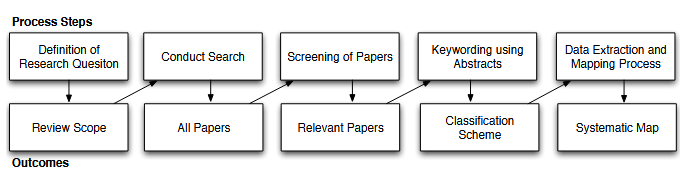
\includegraphics[width=0.8\textwidth]{systematic_mapping_process}
  \caption{The systematic mapping Process}
  \label{fig:systematic_mapping_process}
\end{figure}

